% Created 2018-10-01 Mon 18:53
% Intended LaTeX compiler: pdflatex
\documentclass[conference]{IEEEtran}

\usepackage{graphicx}
\usepackage{amssymb}
\usepackage{amsmath}
\usepackage{xcolor}
\usepackage{url}
\usepackage{listings}
%\usepackage[utf8]{inputenc}
\usepackage[english]{babel}
\usepackage{multirow}
\usepackage{caption}
\usepackage{hyperref}
\usepackage{booktabs}
\usepackage{array}
\usepackage{relsize}
\usepackage{bm}
\usepackage{wasysym}
\usepackage{ragged2e}
\graphicspath{{./img/}}
\renewcommand*{\UrlFont}{\ttfamily\smaller\relax}
\author{\IEEEauthorblockN{Pedro Bruel\IEEEauthorrefmark{1}\IEEEauthorrefmark{2},
Arnaud Legrand\IEEEauthorrefmark{1},
Brice Videau\IEEEauthorrefmark{1} and
Alfredo Goldman\IEEEauthorrefmark{2}}
\IEEEauthorblockA{\IEEEauthorrefmark{1}University of Grenoble Alpes, CNRS, INRIA, LIG - Grenoble, France\\
Email: \{arnaud.legrand, brice.videau\}@imag.fr}
\IEEEauthorblockA{\IEEEauthorrefmark{2}University of São Paulo - São Paulo, Brazil\\
Email: \{phrb, gold\}@ime.usp.br}}
\date{\today}
\title{A Design of Experiments Approach to Autotuning under Tight Budget Constraints}
\hypersetup{
 pdfauthor={},
 pdftitle={A Design of Experiments Approach to Autotuning under Tight Budget Constraints},
 pdfkeywords={},
 pdfsubject={},
 pdfcreator={Emacs 26.1 (Org mode 9.1.14)},
 pdflang={English}}
\begin{document}

\maketitle
\begin{abstract}
Abstract
\end{abstract}

\section{Introduction}
\label{sec:org7ae4f33}
Optimizing code for objectives such as performance and power consumption is
fundamental to the success and cost effectiveness of industrial and scientific
endeavors in High Performance Computing. A considerable amount of highly
specialized time and effort is spent in porting and optimizing code for GPUs,
FPGAs and other hardware accelerators. Experts are also needed to leverage
bleeding edge software improvements in compilers, languages, libraries and
frameworks. The automatic configuration and optimization of High Performance
Computing applications, or \emph{autotuning}, is a technique effective in decreasing
the cost and time needed to adopt efficient hardware and software. Typical
targets for autotuning include algorithm selection, source-to-source
transformations and compiler configuration.

Autotuning can be studied as a search problem, where the objective is to
minimize single or multiple software of hardware metrics. The exploration of the
search spaces defined by configurations and optimizations present interesting
challenges to search strategies. These search spaces grow exponentially with the
number of considered configuration parameters and their possible values. They
are also difficult to extensively explore due to the often prohibitive costs of
hardware utilization and program compilation and execution times. Developing
autotuning strategies capable of producing good optimizations while minimizing
resource utilization is therefore essential. The capability of acquiring
knowledge about an optimization problem is also a desired feature of an
autotuning strategy, since this knowledge can decrease the cost of subsequent
optimizations of the same application or for the same hardware.

It is common and usually effective to use search meta-heuristics such as genetic
algorithms and simulated annealing in autotuning. These strategies usually
attempt to exploit local properties and are not capable of fully exploiting
global search space structures. They are also not much more effective in
comparison with a naive uniform random sample of the search
space~\cite{seymour2008comparison,knijnenburg2003combined}, and usually rely on a
large number of measurements and frequent restarts to achieve good performance
improvements. Search strategies based on gradient descent also are commonly used
in autotuning and rely on a large number of measurements. Their effectiveness
diminishes additionally in search spaces with complex local structures.
Completely automated machine learning autotuning strategies are effective in
building models for predicting important optimization parameters, but still rely
on a sizable data set for training. Large data sets are fundamental to
strategies based on machine learning since they select models from a generally
very large class.

Search strategies based on meta-heuristics, gradient descent and machine
learning require a large number of measurements to be effective, and are usually
incapable of providing knowledge about search spaces to users. At the end of
each autotuning session it is difficult to decide if and where further
exploration is warranted, and impossible to know which parameters are
responsible for the observed improvements. After exploring a search space, it is
impossible to confidently deduce its global properties since its was explored
with unknown biases.

In this paper we propose an autotuning strategy that leverages existing expert
and approximate knowledge about a problem in the form of a performance model,
and refines this initial model iteratively using empirical performance
evaluations, statistical analysis and user input. Our strategy puts a heavy
weight on decreasing the costs of autotuning by using efficient Design of
Experiments strategies to minimize the number of experiments needed to find good
optimizations. Each optimization iteration uses \emph{Analysis of Variance} (ANOVA)
to help identify the relative significance of each configurable parameter to the
performance observations. An architecture- and problem-specific performance
model is built iteratively and with user input, enabling informed decisions on
which regions of the search space are worth exploring.

We present the performance of our approach on a Laplacian Kernel for GPUs where
the search space, global optimum and performance model approximation are known.
The experimental budget on this application were tightly constrained. The
speedups achieved and the budget utilization of our approach on this setting
motivated a more comprehensive performance evaluation. We chose the \emph{Search
Problems in Automatic Performance Tuning}
(SPAPT)~\cite{balaprakash2012spapt} benchmark for this evaluation, where
our approach was able to find speedups of over 50\(\times\) for some SPAPT
applications, finding speedups better than random sampling in some scenarios.
Despite using generic performance models for every SPAPT application, our
approach was able to significantly decrease the budget used to find performance
improvements.

The rest of this paper is organized as follows. Section \ref{sec:orgd95c21a} presents
related work on source-to-source transformation, which is the main optimization
target in SPAPT problems, on autotuning systems and on search space exploration
strategies. Section \ref{sec:org38b9a39} presents a
detailed description of the implementation of our approach and its background.
It discusses the Design of Experiments concepts we incorporate, and the ANOVA
and linear regression algorithms we use in analysis steps. Section \ref{sec:org75da549} presents our results with the GPU Laplacian Kernel and the SPAPT
benchmark. Section \ref{sec:org75230fa} discusses our conclusions and future work.
\section{Background}
\label{sec:orgd95c21a}
\subsection{Source-to-source Transformation}
\label{sec:orgfffd14c}
\subsection{Autotuning}
\label{sec:orgcbb3bc8}
Rice's conceptual framework~\cite{rice1976algorithm} formed the foundation
of autotuners in various problem domains. In 1997, the PHiPAC
system~\cite{bilmes1997optimizing} used code generators and search scripts
to automatically generate high performance code for matrix multiplication. Since
then, systems tackled different domains with a diversity of strategies. Dongarra
\emph{et al.}~\cite{dongarra1998automatically} introduced the ATLAS
project, that optimizes dense matrix multiplication routines. The
OSKI~\cite{vuduc2005oski} library provides automatically tuned kernels for
sparse matrices. The FFTW~\cite{frigo1998fftw} library provides tuned C
subroutines for computing the Discrete Fourier Transform.
Periscope~\cite{gerndt2010automatic} is a distributed online autotuner for
parallel systems and single-node performance. In an effort to provide a common
representation of multiple parallel programming models, the INSIEME compiler
project~\cite{jordan2012multi} implements abstractions for OpenMP, MPI and
OpenCL, and generates optimized parallel code for heterogeneous multi-core
architectures.

Some systems provide generic tools that enable the implementation of autotuners
in various domains. PetaBricks~\cite{ansel2009petabricks} is a language,
compiler and autotuner that introduces abstractions that enable programmers to
define multiple algorithms for the same problem. The ParamILS
framework~\cite{hutter2009paramils} applies stochastic local search methods for
algorithm configuration and parameter tuning. The OpenTuner
framework~\cite{ansel2014opentuner} provides ensembles of techniques that search
spaces of program configurations.
\subsection{Search Space Exploration Strategies}
\label{sec:org6183539}
\section{Applying Design of Experiments to Autotuning}
\label{sec:org38b9a39}
An \emph{experimental design} is a plan for executing a series of experiments
whose objective is to identify the relationships between \emph{factors} and
\emph{responses}. While factors and responses can refer to different concrete
entities in other domains, in computer experiments factors can be configuration
parameters for algorithms and compilers, for example, and responses can be the
execution time or memory consumption of a program.

Experimental designs can be used with various objectives, from identifying the
most important factors to building an analytical model for the response. The
field of Design of Experiments encompasses the mathematical formalization of
the construction of experimental designs. More practical works in the field
present algorithms to generate designs with different objectives and
restrictions.

One of the first detailed descriptions and mathematical treatment of Design of
Experiments was presented by Ronald Fisher~\cite{fisher1937design} in his
1937 book \emph{The Design of Experiments}, where he discussed principles of
experimentation, latin square sampling and factorial designs. Later books such
as the ones from Jain~\cite{bukh1992art},
Montgomery~\cite{montgomery2017design} and Box \emph{et
al.}~\cite{box2005statistics} present comprehensive and detailed
foundations.
\subsection{Design Construction Techniques}
\label{sec:org571b2d6}
Our application of Design of Experiments requires support for factors of
different types and number of possible values, such as binary flags, integer
and floating point numerical values and unordered enumerations of abstract
values. We also need designs that minimize the number of experiments needed for
identifying the most relevant factors in a given problem, since at this moment
we are not interesting in a precise analytical model.

The design construction techniques that fit these requirements are limited.  In
the \emph{2-level screening with random level sampling} technique, factors
with more than two unordered levels are sampled at two random levels. This
enables using small design such as the Plackett-Burman screening design.
Advantages are the small design size and good estimation capability for main
effects. Disadvantages are the incapability of estimating interactions, but
mainly the lack of information regarding the response for levels not selected
in the initial screening.

In \emph{contractive replacement}, an initial 2-Level design is used to
generate mixed-level designs by re-encoding columns into a new single column
representing a multi-level factor. The contractive replacement of
Addelman-Kempthorne is a strategy of this kind.  Advantages are also small
design sizes and good estimation capability of main effects. Additionally, the
contractive replacement technique keeps orthogonality of designs.
Disadvantages are the requirements on the initial designs. Not all 2-Level
designs can be contracted with those methods if orthogonality is desired.

The \emph{direct generation} algorithm presented by Grömping and
Fontana~\cite{ulrike2018algorithm} enables the generation of multi-level
designs with the Generalized Minimum Aberration optimality criterion by solving
mixed integer problems. Advantages are the direct generation of multi-level
designs and the optimality criteria. Disadvantages are the use of proprietary
MIP solvers and the limitations on the size and shape of the designs that can be
generated.
\subsection{D-Optimal Designs}
\label{sec:org118aa47}
The best candidate we have found so far are \emph{D-Optimal} designs. Considering
that we are going to analyse the results of an experiments plan, the
\emph{D-Efficiency} of a design is inversely proportional to the \emph{geometric mean} of
the \emph{eigenvalues} of the plan's \emph{covariance matrix}. A D-Optimal design has the
best D-Efficiency. Our current approach is based on D-Optimal designs.
\subsection{ANOVA}
\label{sec:orgf287022}
\subsection{The DLMT Strategy}
\label{sec:orge3c5fe6}
\begin{center}
\begin{center}
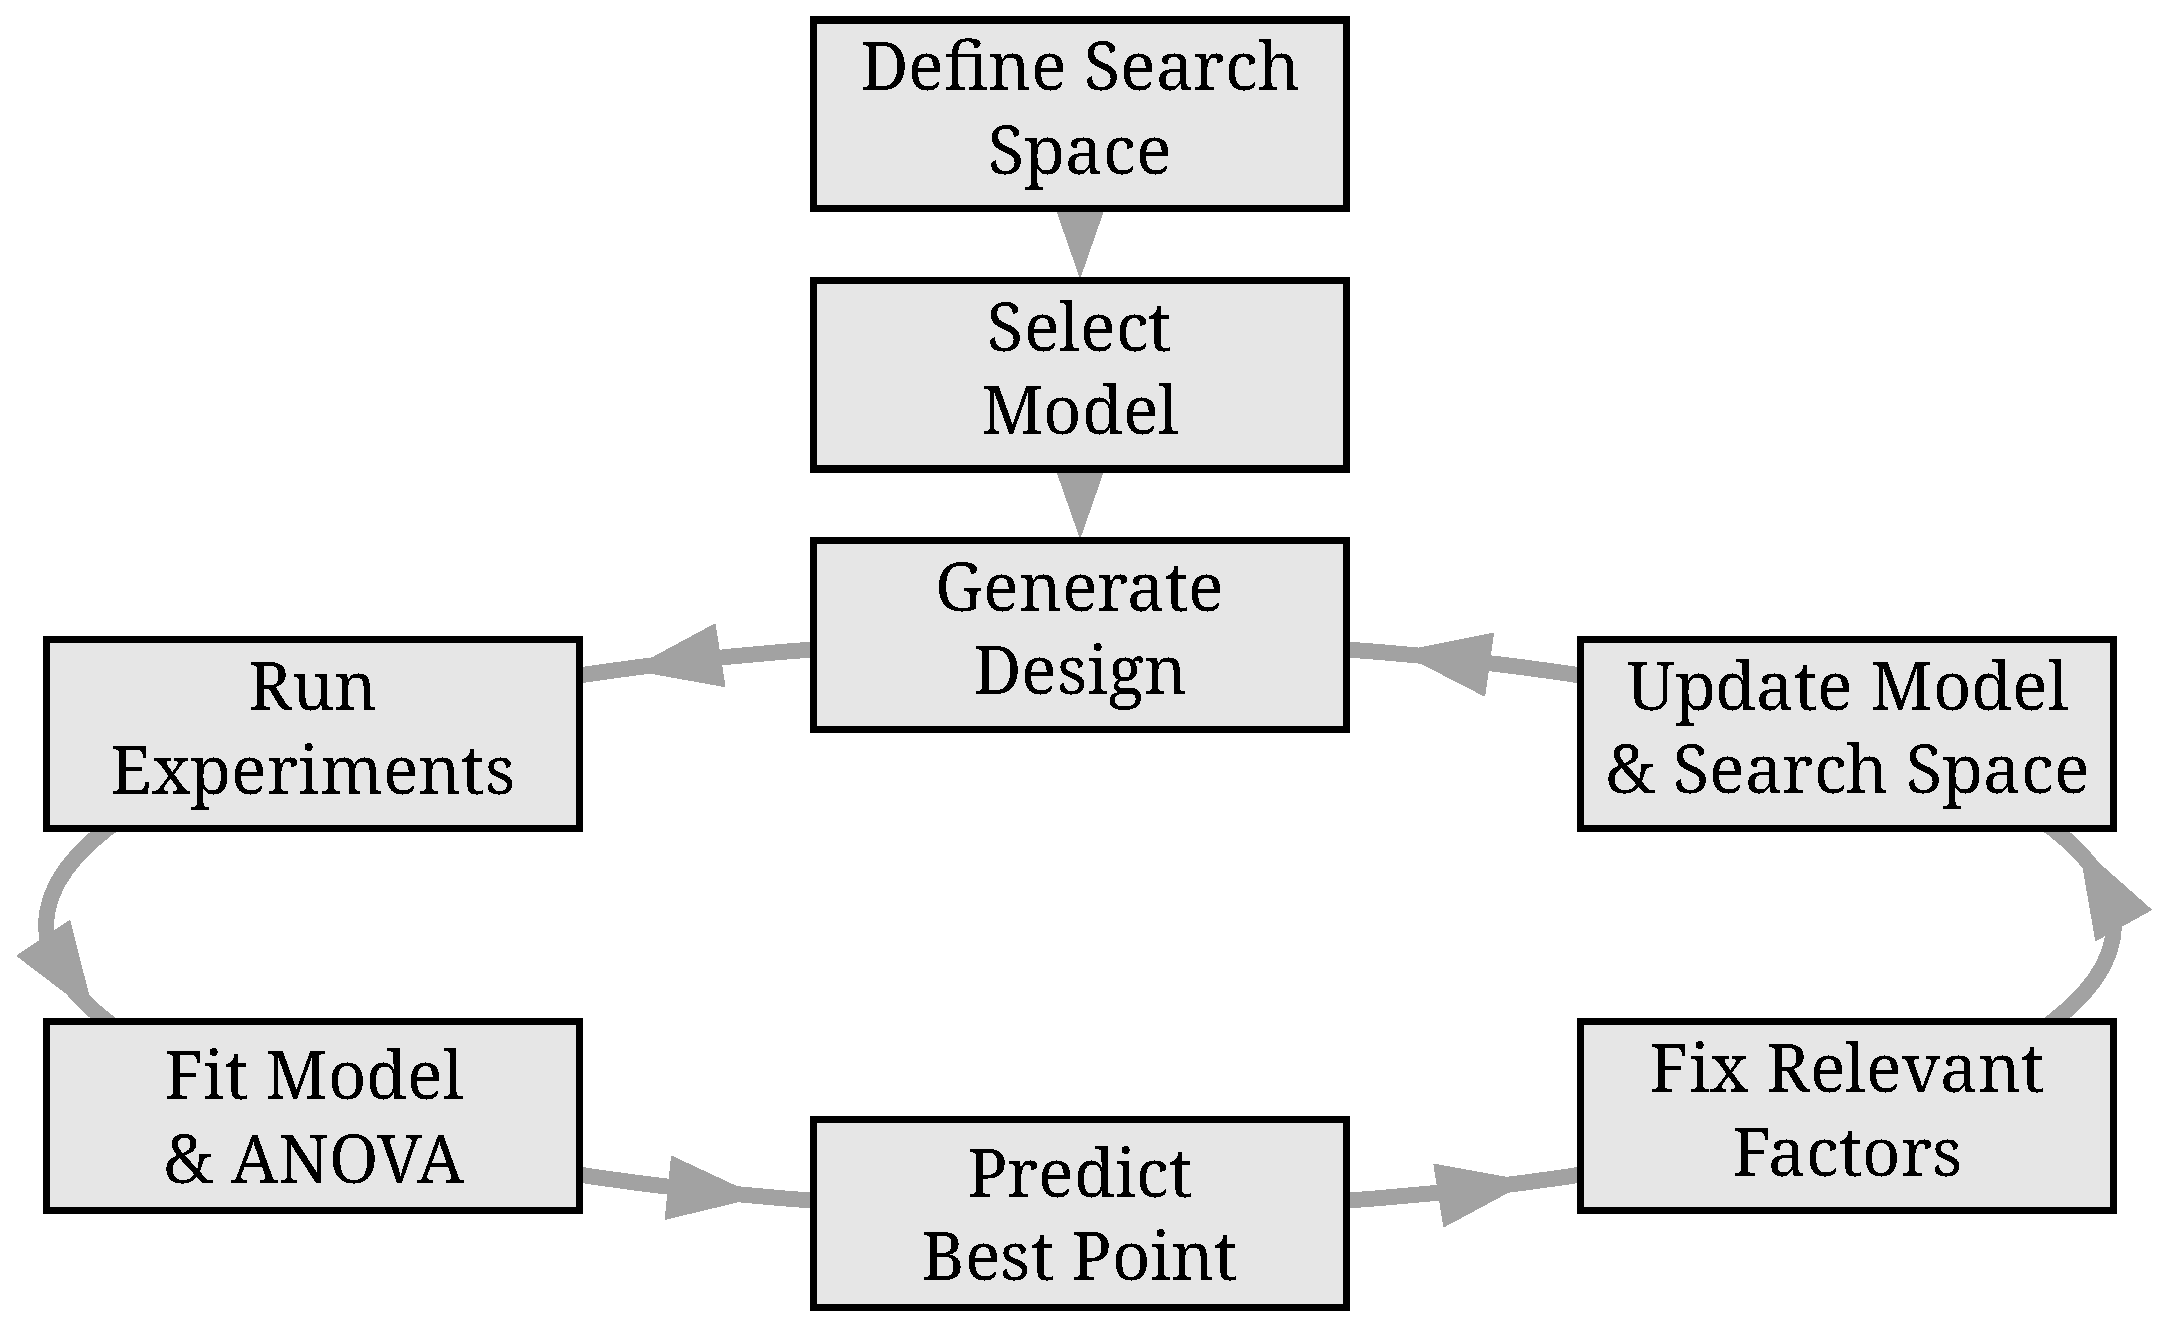
\includegraphics[width=.8\columnwidth]{./img/doe_anova_strategy.eps}
\end{center}
\end{center}

\section{Performance Evaluations}
\label{sec:org75da549}
\subsection{Example on a GPU Laplacian Kernel}
\label{sec:org46366b2}
\subsection{Results on the SPAPT Benchmark}
\label{sec:org4af1fd7}
\subsubsection{Experimental Methodology}
\label{sec:org05faa84}
\section{Conclusion}
\label{sec:org75230fa}
\section*{Acknowledgment}
\label{sec:org1d70f6b}
\bibliographystyle{IEEEtran}
\bibliography{references}
\end{document}
